\chapter{Models and Simulations}

A simulation is intended to imitate in many cases, a real-world process or system, that may be too difficult or costly to analyze directly. Before any such simulation can begin, a model of the system studied must be constructed. Models capture the characteristics and behaviours of the system they represent and in general, a model should be as simple as possible (since resources are limited) while still explaining experimental observations and making predictions with a given degree of accuracy. The simulation is the implementation of the model and can be executed on a computer to produce data for testing, analysis, and visual presentation.

In our simplified model of a biological tissue, the relatively ordered and periodic nature of cells in most simple tissues is captured as a series of repeating \textit{unit cells}. These unit cells are the building blocks of the heterogeneous 1D and 2D models. Each unit cell is characterized by a cellular domain, separated from an extracellular domain by a semi-permeable membrane. The domains are isotropic except at the boundaries where a change in viscosity and semi-permeable barrier exist. Within each domain, the only characteristic modelled is viscosity, and is implemented as a directional stepping probability (Section \ref{sec:intro-diffusion}). Regarding the boundaries, there exists two kinds in our models. The first kind is a totally-reflecting boundary; it forms the absolute boundary of the model system and represents an insurmountable physical barrier. The second kind is a semi-permeable non-active/passive boundary and represents the selectively permeable nature of the plasma membrane. In a real biological plasma membrane, the integral membrane proteins can facilitate either active or passive transport. In the simple cell model developed, the semi-permeable membranes behave in a passive transport manner and this is implemented as a boundary transition probability, a concept explained in Section \ref{sec:intro-diffusion}.

The diffusion of idealized particles, which are non-interacting, experience no net force, and boundary constraints . Particle motion is therefore undirected but occurs in only 1 direction (along a line) in the 1D system, and in 2 orthogonal directions in the 2D system. It was decided from the start that a fixed particle jump/step-size, compared to a Gaussian step-size, would yield data sufficiently accurate for our analytical purposes.

\begin{figure}[h]
	\centering
	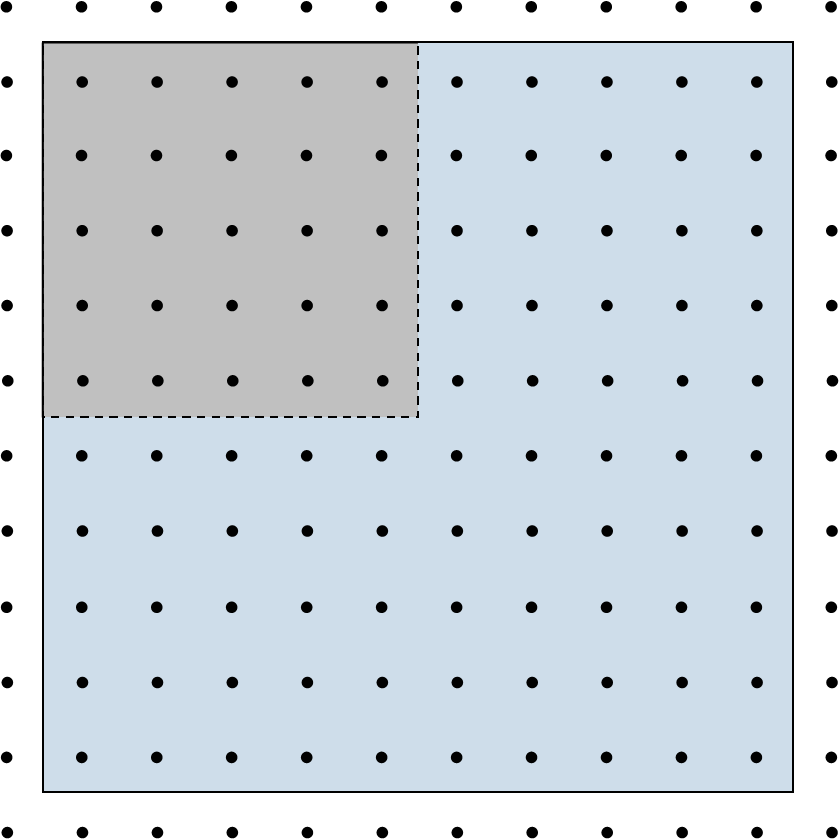
\includegraphics[width=0.5\linewidth]{2d_unit_cell_1.png}
	\caption{A single 2D unit cell forms the building block of the 2D model. An example lattice arrangement is overlayed on the model to show possible particle positions. The dimensions of each domain can be adjusted individually by increasing or decreasing the number of lattice points used in the simulation. Dashed lines represent semi-permeable boundaries and lattice points outside the cell belong to adjacent cells.}
	\label{fig:2d_unit_cell_1.png}
\end{figure}

Particle diffusion in both the 1D and 2D systems were simulated using Monte Carlo and master equation approaches. 

Using Monte Carlo, information on the individual state (i.e. current position and path history) can be maintained. However, due to the finite number of particles used in the simulation and the stochastic nature of individual particle motion, statistical fluctuations lead discontinuous (?) distributions.

Using the master equation methods and evolving the particle density distribution in time, discontinuations (?) in the distributions are no longer an issue, however at the expense of no information on individual particle state.

For both simulation types, the computed density distribution at every time step was written to a file. From the data generated, information such as mean particle (ensemble?) position was extracted for computation of the mean-square-displacement at every time step.

The density distribution data was also turned into visual graphic that could show the evolution of the particle diffusion within the system, in time.

\section{1-Dimensional Systems}
In 1D, homogenous and heterogeneous simple cell systems were simulated using Monte Carlo (MC) and master equation approaches. 



\subsection{Homogenous System}


*include figure of homogenous model*

\subsection{Heterogeneous System}


\begin{figure}[h]
	\centering
	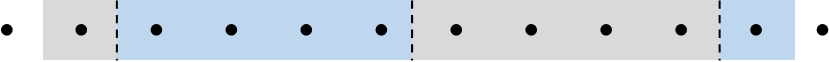
\includegraphics[width=1.0\linewidth]{1d_unit_cell_2.png}
	\caption{2D lattice unit cell with cellular and extracellular regions. Dashed lines indicate semi-permeable barrier.}
	\label{fig:1d_unit_cell_2.png}
\end{figure}

\section{2-Dimensional System}

\begin{figure}[h]
	\centering
	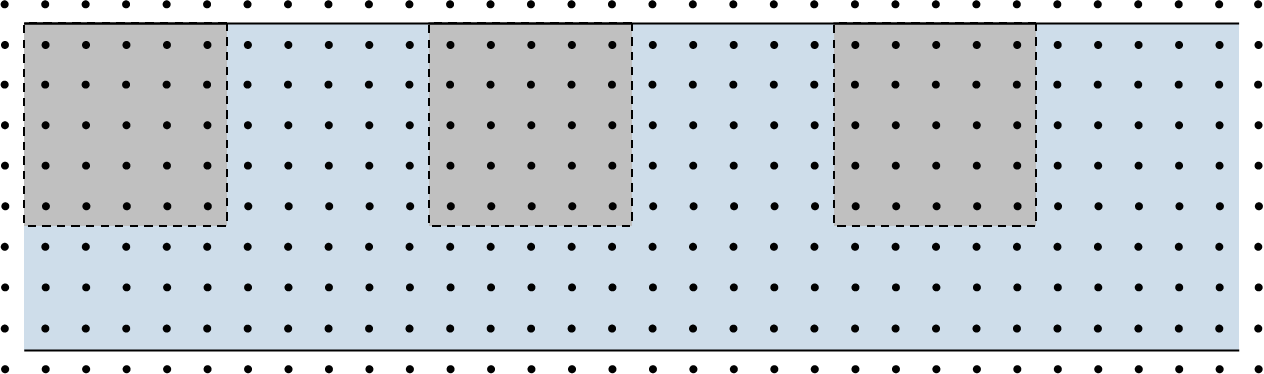
\includegraphics[width=1.0\linewidth]{2d_unit_cell_2.png}
	\caption{2D lattice unit cell with cellular and extracellular regions. Dashed lines indicate semi-permeable barrier.}
	\label{fig:2d_unit_cell_2.png}
\end{figure}
*include figure of heterogeneous model*